\documentclass{memoir}
\usepackage{graphics}
\usepackage{hyperref}
\usepackage{listings}
\usepackage{color}
\usepackage{makeidx}
\usepackage[acronym,toc]{glossaries}
\usepackage{longtable}
\usepackage{todonotes}

\newacronym{acronym:GNU}{GNU}{GNU is Not Unix}

\newglossaryentry{agile}
{
    name=agile,
    description={
        A style of organizing software development described by the Agile Manifesto.
    }
}


\makeindex
\makeglossaries

\title{Title of the Book}
\date{2020-12-13}
\author{Your Name}

\stockaiv

\begin{document}
\frontmatter
\pagenumbering{roman}
\maketitle
\newpage
\tableofcontents
\newpage
\listoffigures
\newpage
\listoftables
\newpage
\lstlistoflistings
\include{chapters/preface}

\mainmatter
\part{Introduction}
\chapter{Introduction to C}
\epigraph{``C is quirky, flawed, and an enormous success.''}{\em Dennis M. Ritchie\index{Ritchie, Dennis M.}\em}

The C Programming Language, short ``C'', was developed by \index{Ritchie, Dennis M.}Dennis M. Ritchie.

C first appeared in 1972, which makes it quite an old language by today's standards.
Despite its age, C still is in widespread use, and will remain so for the foreseeable future.

The major fields of application for C include:
\begin{itemize}
\item \Gls{firmware}
\item Operating system kernels
\item Drivers
\item Basic operating system utilities and programs
\item Core of virtual machines, runtime environments, and interpreters
\end{itemize}

C was made popular with the book ``The C Programming Language''\cite{kernighanAndRitchie} by \index{Kernighan, Brian}Brian Kernighan and \index{Ritchie, Dennis M.}Dennis M. Ritchie.
This book is often referred to under the name ``The Kernighan \& Ritchie''.
It has made it famous and popular to introduce a programming language with a very simple first listing that displays the message ``Hello, world!'' on the screen.

\lstinputlisting[caption={\index{Hello, World!C}Hello, World! in C}, label={lst:hello.c}]{src/hello.c}

The C Programming Language is the language in which Linux is written.
It is also the language of much of the \acrshort{acronym:GNU} software.

\chapter{Text Editors}
\epigraph{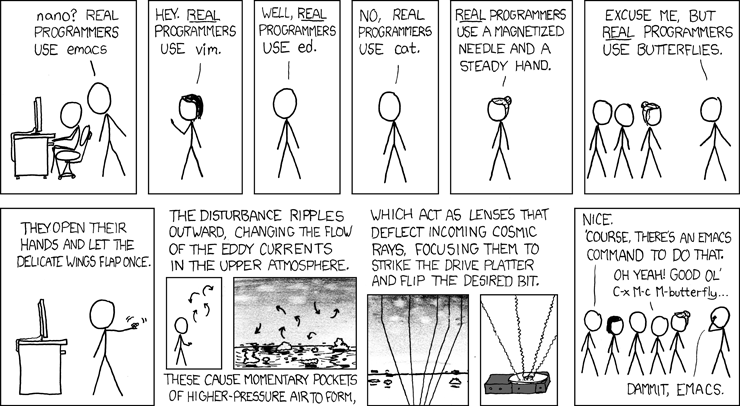
\includegraphics[width=\textwidth]{gfx/real_programmers}}{xkcd}

\part{Integration}
%\include{chapters/part2/chapter3}
%\include{chapters/part2/chapter4}

\appendix
\part{Appendix}
\chapter{Hardware Used}
For the creation of this template, the following hardware was used:
\begin{itemize}
\item \index{Razer}Razer Blade Stealth, Intel\textsuperscript{®} Core™ i7-8550U, 16 GiB RAM, 512 GB SSD
\item Razer Core V2, ASUS ROG Nvidia GeForce GTX 1070 GPU
\item 4 LG24UD58 screens (4K resolution 3840×2160)
\item \index{Microsoft}Microsoft Sculpt Ergonomic Keyboard for Business and Razer Lancehead mouse
\item Razer Leviathan speakers and Razer Seirēn Pro microphone
\item Razer Stargazer, Razer Kiyo, and \index{Logitech}Logitech C920 webcams
\end{itemize}

\begin{figure}
\caption{My desk}
\centering
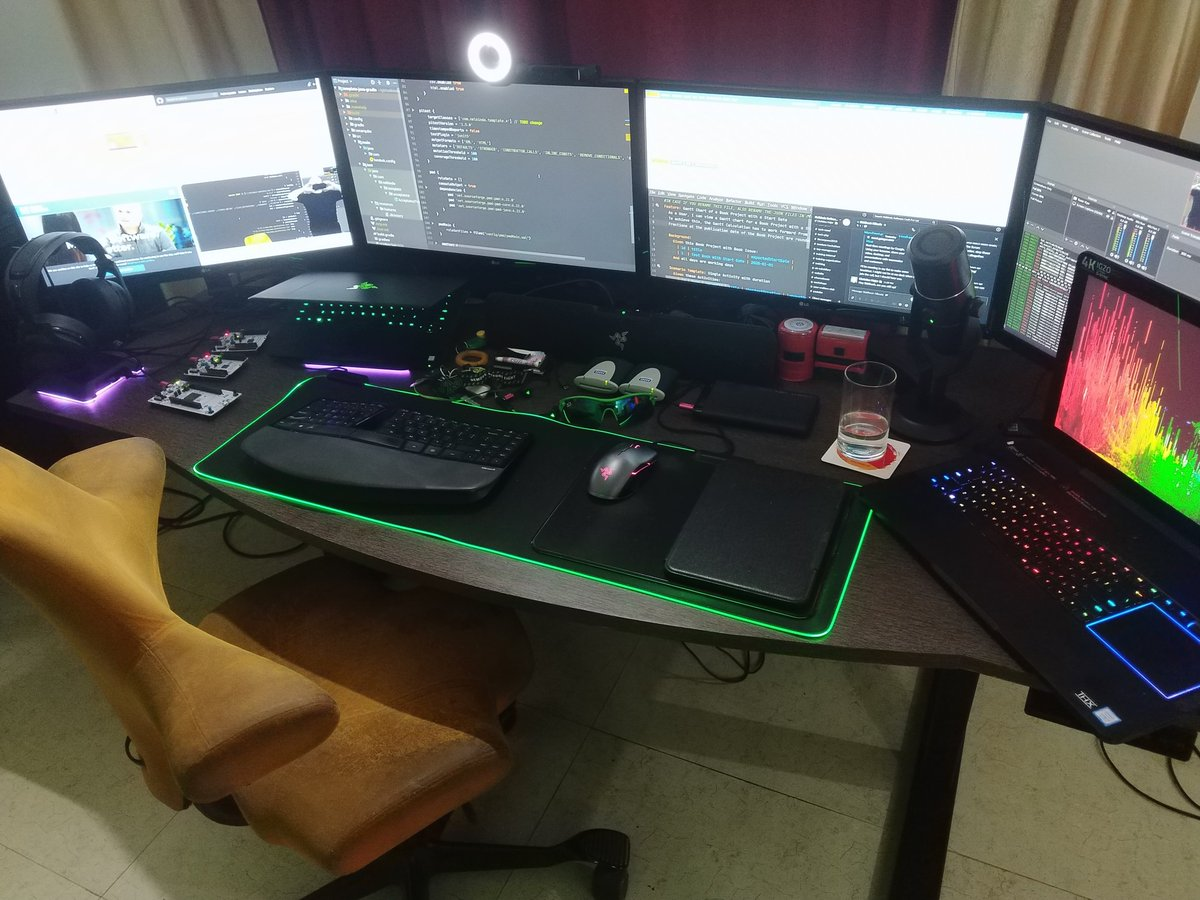
\includegraphics[scale=0.2]{gfx/desk}
\end{figure}

\chapter{Some Unicode Symbols}
The table \ref{unicodeSymbols} lists a few unicode characters that work with this book template.

\begin{table}[h]
\centering
\begin{tabular}{|c c c c|}
\hline
Hex & Decimal & Symbol & Name \\
\hline\hline
A9 & 169 & © & Copyright \\
2122 & 8482 & ™ & Unregistered Trademark \\
2026 & 8230 & … & horizontal ellipsis \\
\hline
\end{tabular}
\caption{Table of some unicode symbols}
\label{unicodeSymbols}
\end{table}


\backmatter
\printglossary[type=\acronymtype]
\printglossary
\bibliographystyle{ieeetr}
\bibliography{data/book}
\printindex
\end{document}
